% !TEX root = manuscript.tex
\glsresetall[\acronymtype]
%\addbibresource{../resource/ref.bib}
\chapter{Conceptual Framework}%\chapter{Key Features of \acs{3GPP} \acs{5G} Standards}%\chapter{\acs{5G} Scenario}%{System Modeling}
\label{chp:theory}

This chapter provides some basic concepts that serve as a background to the subsequent chapters.
%
The chapter is divided into two parts.
%
First, we provide a brief overview on physical layer procedures for downlink data transmission in \gls{5g} \gls{nr}.
%
Then, some fundamental concepts of \gls{rl} are briefly surveyed.
%
% This chapter is divided into two parts, in each one we give an overview of a subject, mainly:
% \begin{enumerate}
%     \item The first part will give an overview of the transmission of downlink data, as well as some of the \gls{phy} procedures associated with it.
%     \item The second part will give an overview of some fundamental concepts of \gls{rl}.
% \end{enumerate}

\section{Transmission Procedures}
\label{sec:5gnr-trans}
% Transport Channel Processing on 5G NR
\Gls{mac} uses services from the physical layer in the form of transport channels.
%
A transport channel defines how the information is transmitted over the radio interface \cite{3gpp.38.212} \cite{ErikDahlman5G}.
%
The transport channels defined for 5G-NR in the downlink are the \gls{dlsch}, the \gls{pch}, and the \gls{bch}.
%
In the uplink, there are two transport channels, the \gls{ulsch} and the \gls{rach}.
% Downlink transmissions make use of  \gls{dlsch}, \gls{pch} and \gls{bch}. In the uplink, the transport channel is called \gls{ulsch}.
%
% The data transmissions in the downlink use the \gls{dlsch} and in the uplink the \gls{ulsch} \cite{AliZaidi632018}.
Downlink data uses the \gls{dlsch}, while the uplink uses the \gls{ulsch} \cite{AliZaidi632018}.
%

Each transport channel is mapped to some physical channel, with a physical channel corresponding to a set of time-frequency resources used for transmission.
%
This transmission can be of transport channel data, control information, or indicator information.
%
The physical channels without the corresponding transport channel are used for conveying the \gls{dci} and \gls{uci} \cite{ErikDahlman5G}.
%
The physical channels defined for \gls{5g} \gls{nr} are \cite{3gpp.38.211}:

\begin{enumerate}
    \item \Gls{pdsch}: used not only for downlink data transmission, but also for random-access response messages, parts of the system information and paging information.
    %
    \item \Gls{pdcch}: used for \gls{dci}, that includes scheduling decisions needed for the reception of downlink data and scheduling grants for uplink data transmission.
    %
    \item \Gls{pbch}: used to broadcast system information needed by the device to access the network.
    %
    \item \Gls{pusch}: used for uplink data transmission.
    %
    \item \Gls{pucch}: used for \gls{uci}, which includes \gls{harq} acknowledgments, scheduling request and downlink \gls{csi}.
    %
    \item \Gls{prach}: used for random access.
\end{enumerate}

The mapping of transport channels and control information to physical channels is depicted in Figure \ref{fig:channel-mapping}.

\begin{figure}[htbp]
    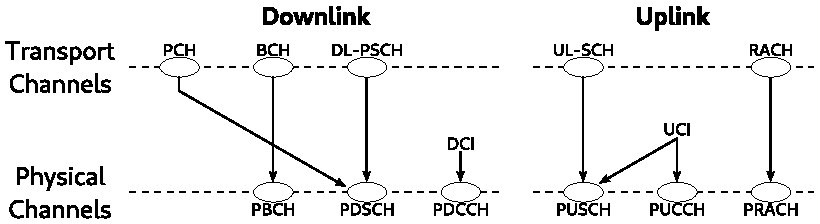
\includegraphics[width=0.95\columnwidth]{figures/chp_theory/complete.pdf}
    \caption{Mapping of transport channels to physical channels}
    \source{Created by the author based on \cite{ErikDahlman5G}}
    \label{fig:channel-mapping}
\end{figure}


Data in the transport channel is organized into transport blocks. For each component carrier and at each \gls{tti}, up to two \glspl{tb} are conveyed to the physical layer and transmitted over the radio interface  \cite{ErikDahlman5G}.
%
The transmission process is summarized in Figure \ref{fig:transmission}.
%
This process is similar for the uplink and downlink, the only difference being the additional step of transform precoding after the layer mapping in the uplink case.

\begin{figure}[htbp]
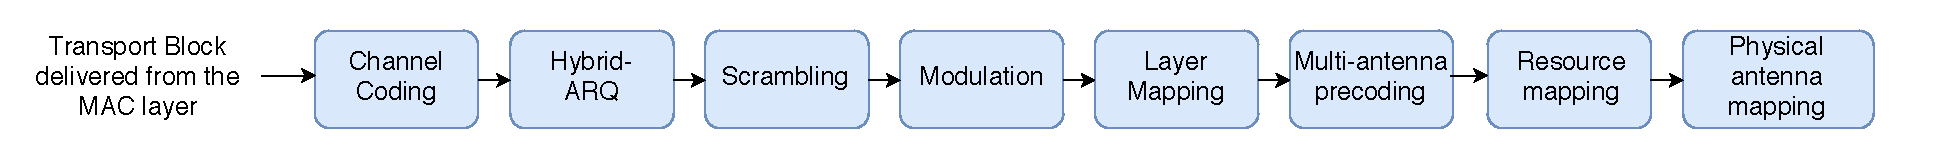
\includegraphics[width=\columnwidth]{figures/chp_theory/transmissionmodel.pdf}
% \caption{General transmission model on \gls{5g} \gls{nr}}
\caption{General transport-channel processing on \gls{5g} \gls{nr}}
\label{fig:transmission}
\end{figure}
%
In the modulation phase, \gls{nr} supports \gls{qpsk} and three orders of \gls{qam}, namely 16\gls{qam}, 64\gls{qam} and 256\gls{qam}, for both the uplink and downlink, with an additional option of $\pi/2$-BPSK in the uplink.
%
The \gls{fec} code for the \gls{embb} use case in data transmission is the \gls{ldpc} code, whereas in the control signaling polar codes are used.
%

\begin{figure}[htbp]
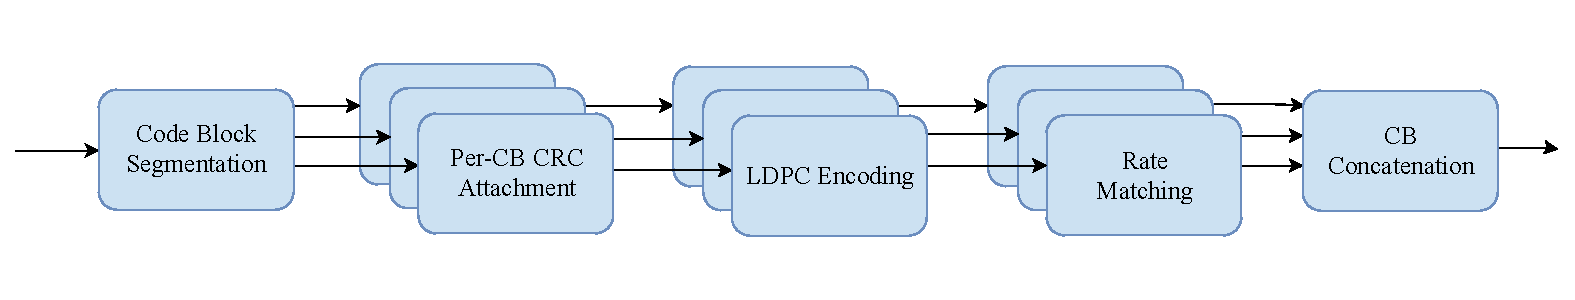
\includegraphics[width=\columnwidth]{figures/chp_theory/channelcoding.pdf}
\caption{\gls{ldpc} channel coding procedure on \gls{5g} \gls{nr}}
\label{fig:channel-coding}
\end{figure}

In our work, we are mainly concerned with the \gls{pdsch}, since the data is transmitted from the \gls{bs} to the \gls{ue}.
%
In this case the overall \gls{5g} \gls{nr} channel coding process comprises six steps, as shown in Figure \ref{fig:channel-coding} \cite{ErikDahlman5G}, namely:
\begin{itemize}
	\item \Gls{crc} Attachment: Calculates a \gls{crc} and attaches it to each transport block. It facilitates error detection and its size can be of 16 bits or 24 bits.
	\item Code-block segmentation: Segments the transport block if it is larger than the size supported by the \gls{ldpc} encoder. Produces \gls{cb} of equal size.
	\item Per-\gls{cb} \gls{crc} Attachment: A \gls{crc} is calculated and appended to each \gls{cb}.
	\item \gls{ldpc} Encoding: The solution used in \gls{nr} is a Quasi-cyclic \gls{ldpc} with two base graphs, that are used to build the different parity-check matrices with different payloads and rates.
	\item Rate Matching: It adjusts the coding to the allocated resources. It consists of bit selection and bit interleaving.
	\item Code-Block Concatenation: Concatenates the multiple rate-matching outputs into one block.
\end{itemize}

The other blocks in Figure \ref{fig:transmission}, excluding the channel coding and the modulation, are:
\begin{enumerate}
	\item \Gls{harq}: \gls{5g} \gls{nr} uses \gls{harq} with soft combining as the primary way to handle retransmissions. In this approach, a buffer is used to store the erroneous packet and this packet is combined with the retransmission to acquire a combined packet, which is more reliable than its components.
	%
	\item Scrambling: The process of scrambling is applied to the bits delivered by the \gls{harq}. Scrambling helps in the mitigation of the effects the interference by the \gls{fec}.
	%
	\item Layer mapping: The process of layer mapping is applied to the modulated symbols. It distributes the symbols across different transmission layers.
	%
	\item Multi-antenna precoding: This step uses a precoder matrix to map the transmission layers to a set of antenna ports.
	%
	\item Resource mapping: This process takes the symbols that should be transmitted by each antenna port and maps these to the set of available resource elements.
	%
	\item Physical antenna mapping: Maps each resource to a physical antenna.
\end{enumerate}

The \gls{pdsch} has only one defined transmission scheme \cite{3gpp.38.214}.
%
In this scheme the downlink transmission can be performed with up to 8 transmission layers on antenna ports 1000-1011.
%


In the following subsections we give an overview of the \gls{5g} \gls{nr} \gls{ldpc} coding solution and a more detailed explanation of some of the \gls{pdsch} procedures in Figure \ref{fig:transmission}.


%%%%%%%%%%%%%%%%%%%%%%%%%%%%%--subsection--%%%%%%%%%%%%%%%%%%%%%%%%%%%%%%%%%


\subsection{\Acl{mcs} and \acl{tbs} determination}

To start the decoding process, the \gls{ue} must first determine the modulation order, the target code rate and the \glspl{tbs} in the \gls{pdsch}.
%
To this end, the \gls{ue} needs some information:

\begin{enumerate}
    \item The \gls{mcs} index, $I_{mcs}$, which is a 5-bit field in the \gls{dci}.
    %
    \item The redundancy version, which is used for the \gls{harq} functionality on the rate-matching step of the channel coding and is a 2-bit field included in the \gls{dci}.
    %
    \item The number of transmission (spatial multiplexing) layers.
    \item The number of allocated \glspl{prb} before the rate matching.
\end{enumerate}

The \gls{mcs} index is used alongside a table to determine the modulation order and the target code rate.
%
Until the writing of this work only three \gls{mcs} tables were defined in the the technical specification \cite{3gpp.38.214}, two of modulation order up to 64\gls{qam}, with one of those used for a low spectral efficiency case, and one with modulation order going up to 256\gls{qam}.
%
In this work, we used the table \cite[Table 5.1.3.1-2]{3gpp.38.214}, that goes up to 256\gls{qam}, reproduced in Table \ref{tab:mcs-table}, where \gls{not:rate} is the target code rate:

\begin{table}[htb]
\centering
\caption{\gls{mcs} index table 2 for \gls{pdsch}}
\label{tab:mcs-table}
\begin{tabularx}{0.95\columnwidth}{l X X r}
  \toprule
  \gls{mcs} index  & Modulation order & \gls{not:rate} x 1024  &  Spectral efficiency \\
  \midrule
  0  &  2   & 120       &  0.2344 \\
  1  &  2   & 193       &  0.3770 \\
  2  &  2   & 308       &  0.6016 \\
  3  &  2   & 449       &  0.8770 \\
  4  &  2   & 602       &  1.1758 \\
  5  &  4   & 378       &  1.4766 \\
  6  &  4   & 434       &  1.6953 \\
  7  &  4   & 490       &  1.9141 \\
  8  &  4   & 553       &  2.1602 \\
  9  &  4   & 616       &  2.4063 \\
  10 &  4   & 658       &  2.5703 \\
  11 &  6   & 466       &  2.7305 \\
  12 &  6   & 517       &  3.0293 \\
  13 &  6   & 567       &  3.3223 \\
  14 &  6   & 616       &  3.6094 \\
  15 &  6   & 666       &  3.9023 \\
  16 &  6   & 719       &  4.2129 \\
  17 &  6   & 772       &  4.5234 \\
  18 &  6   & 822       &  4.8164 \\
  19 &  6   & 873       &  5.1152 \\
  20 &  8   & 682.5     &  5.3320 \\
  21 &  8   & 711       &  5.5547 \\
  22 &  8   & 754       &  5.8906 \\
  23 &  8   & 797       &  6.2266 \\
  24 &  8   & 841       &  6.5703 \\
  25 &  8   & 885       &  6.9141 \\
  26 &  8   & 916.5     &  7.1602 \\
  27 &  8   & 948       &  7.4063 \\
  28 &  2   & Reserved  & Reserved \\
  29 &  4   & Reserved  & Reserved \\
  30 &  6   & Reserved  & Reserved \\
  31 &  8   & Reserved  & Reserved \\
  \bottomrule
\end{tabularx}
\source{\cite[Table 5.1.3.1-2]{3gpp.38.214}}
\end{table}

The \gls{tbs} determination process is defined in \cite[Section 5.1.3.2]{3gpp.38.214}, and it depends on the following parameters:

\begin{enumerate}
    \item $N_{\text{sc}}^{\text{RB}}$: The number of subcarriers in a \gls{rb}, 12.
    \item $N_{\text{symb}}^{\text{sh}}$: Number of symbols of the \gls{pdsch} allocation within the slot.
    \item $N_{\text{DMRS}}^{\text{PRB}}$: Number of \glspl{re} for \gls{dmrs} per \gls{prb} in the scheduled duration including the overhead of the \gls{dmrs} \gls{cdm} groups without data.
    \item $N_{\text{oh}}^{\text{PRB}}$: Overhead configured by a higher layer parameter. Set to 0 if not configured.
    \item $n_{\text{PRB}}$: Total number of allocated \glspl{prb} for the \gls{ue}.
\end{enumerate}

With the above information, the total number of \glspl{re} in the \gls{pdsch} allocation can be determined, which will be used to calculate the \gls{tbs} using also the number of transmission layers, \gls{not:nLayers}, the target code rate, \gls{not:rate}, and the modulation order, \gls{not:mod}.

At the transmitter side, \gls{bs}, a \gls{tb} of size \gls{tbs} is delivered from the \gls{mac} to the \gls{phy} where the process of Figure \ref{fig:transmission} happens.

%%%%%%%%%%%%%%%%%%%%%%%%%%%%%--subsection--%%%%%%%%%%%%%%%%%%%%%%%%%%%%%%%%%


\subsection{The \gls{5g} \gls{nr} \gls{ldpc}}
\label{subsec:ldpc}

Before explaining the procedures in Figure \ref{fig:transmission}, we give an introduction to the \gls{ldpc} solution applied to the \gls{embb} use case in the \gls{5g} \gls{nr}.
%

\Gls{ldpc} codes are a class of linear block codes based on a sparse \gls{pcm}  originally proposed by Gallager \cite{gallager1962}.
%
Several standards have incorporated \gls{ldpc} codes, such as IEEE 802.11n, IEEE 802.16e (WiMAX) and \gls{dvb-s2} \cite{AliZaidi632018}.
%
In the third and forth generations (3G and 4G), turbo codes were the primary coding scheme \cite{Richardson2018}.
%
It has also been considered as a candidate for the \gls{5g} \gls{nr} along with polar codes and \gls{ldpc} codes \cite{Hamidi8417496}.
%
The \gls{5g} \gls{nr} will make a transition on the error correcting codes with the \gls{ldpc} codes being used for the data channel and polar codes being used for the control information, on both the \gls{embb} and in the release-15 \gls{urllc} use cases \cite{bae_abotabl_lin_song_lee_2019}.

Although turbo codes and \gls{ldpc} codes have similar error-correcting capabilities \cite{ErikDahlman5G}, \gls{ldpc} codes provide the following advantages \cite{Hui2018}:

\begin{enumerate}
    \item Higher coding gains
    \item Lower error floors
    \item Higher achievable peak throughput
    \item Lower decoding complexity and improved decoding latency, particularly on high code rates
    \item Can achieve greater parallelism in the decoding process
\end{enumerate}

In a $(\gls{not:coded-bits}, \gls{not:info-bits})$ \gls{ldpc} code, the \gls{pcm} is a $ (\gls{not:coded-bits}-\gls{not:info-bits}) \times n$ sparse matrix, with $\gls{not:info-bits}$ being the number of information bits and $\gls{not:coded-bits}$ being the number of code-word bits, i.e information bits plus parity bits.
%
The sparseness of the \gls{pcm} enables a relatively simple decoding by making use of low-complexity iterative decoding algorithms.


The \gls{pcm} can also be represented by a graph connecting $\gls{not:coded-bits}$ variable nodes with $(\gls{not:coded-bits}-\gls{not:info-bits})$ check nodes, the check nodes correspond to the parity-check equations.
%
In this graph, there is an edge between a variable node and a check node if the corresponding entry on the \gls{pcm} is not-null \cite{Richardson2018}.
%
This bipartite graph representation is known as the Tanner graph \cite{TannerGraph} and is the reason that the term \glsfirst{bg} is used in the \gls{nr} specifications.
%


The \gls{nr} \gls{ldpc} codes are \gls{qc} \gls{ldpc} codes, a class of photograph codes \cite{bae_abotabl_lin_song_lee_2019}.
%
In \gls{qc}-\gls{ldpc} the \gls{pcm} is constructed based on a smaller photograph, also called base matrix or \gls{bg}, that describes the macroscopic structure of the code \cite{Richardson2018}.
%
The \gls{pcm} can then be constructed by replacing each entry of the base matrix by a $\gls{not:lift-factor} \times \gls{not:lift-factor} $ cyclic permutation matrix.
%
This process is called lifting and $\gls{not:lift-factor}$ is the lifting size \cite{AliZaidi632018}.


In a Tanner graph representation, the lifting procedure is equivalent to having the larger graph being formed by $\gls{not:lift-factor}$ copies of the \gls{bg} and permuting the edges, as shown in Figure \ref{fig:graph-lifting}.
%
One important consequence of this structure is that, with the higher possible parallelism, the decode complexity is a function of the \gls{bg} size, not of the actual \gls{pcm} size, since a degree of parallelism of $\gls{not:lift-factor}$ can be achieved \cite{bae_abotabl_lin_song_lee_2019}.
% The \gls{nr} specifies the maximum $\gls{not:lift-factor}$ to $384$.

\begin{figure}[htbp]
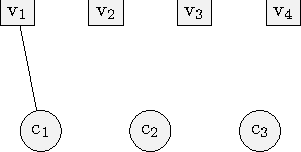
\includegraphics[width=\columnwidth]{figures/chp_theory/tanner_graph.pdf}
\caption{Construction of a larger graph from a base graph using a lifting size of 2}
\label{fig:graph-lifting}
\end{figure}


In the \gls{5g} \gls{nr} \gls{ldpc} code, each ``0'' in the \gls{bg} is replaced by a $\gls{not:lift-factor} \times \gls{not:lift-factor} $ all-zero matrix and each ``1'' is replaced by a circularly shifted identity matrix, shifted by the corresponding shifting coefficient, \gls{not:shift-coef}, \cite{ErikDahlman5G}.
%
In the technical specification \cite{3gpp.38.212}, 51 lifting sizes are specified and they are divided in 8 groups, called set index $\gls{not:set-index}$.
%
Each set index corresponds to a different permutation design, i.e different shifting coefficients, as summarized in Table \ref{tab:lift-table}.
%
This design means that there are 51 \glspl{pcm} for each of the two \glspl{bg}.

\begin{table}[htb]
\centering
\caption{Sets of \gls{ldpc} lifting sizes}
\label{tab:lift-table}
\begin{tabular}{l c}
  \toprule
  Set index $\gls{not:set-index}$   & Set of lifting sizes $\gls{not:lift-factor}$ \\
  \midrule
  0  &  2, 4, 8, 16, 32, 64, 128, 256 \\
  1  &  3, 6, 12, 24, 48, 96, 192, 384 \\
  2  &  5, 10, 20, 40, 80, 160, 320 \\
  3  &  7, 14, 28, 56, 112, 224 \\
  4  &  9, 18, 36, 72, 144, 288 \\
  5  &  11, 22, 44, 88, 176, 352 \\
  6  &  13, 26, 52, 104, 208 \\
  7  &  15, 30, 60, 120, 240 \\
  \bottomrule
\end{tabular}
\source{\cite[Table 5.3.2-1]{3gpp.38.212}}
\end{table}


Two \glspl{bg} are specified in \gls{5g} \gls{nr}, in order to guarantee efficiency for all the payload sizes and code rates.
%
The \gls{bg}1 has dimensions of $46 \times 68$, meaning 22 systematic columns, while \gls{bg}2 has dimensions of $42 \times 52$, which converts to 10 systematic columns.
%
The first 2 columns of the \gls{bg}, which correspond to the first $2 \gls{not:lift-factor}$ columns in the \gls{pcm} are punctured, meaning that the corresponding bits are not actually transmitted, but need to be recovered at the receiver.
%
\Gls{bg}2 is designed to low code rates, between $1/5$ and $5/6$ and shorter information block sizes, up to 3840, whereas \gls{bg}1 is used for larger information block sizes, up to 8448, and higher code rates, between $1/3$ and $22/24$.
%
\Gls{cb} segmentation is used whenever \gls{not:info-bits} is larger than the maximum designed information block size.
%
Puncturing can increase the highest code rate while repetition can be used to achieve lower code rates \cite{ErikDahlman5G,AliZaidi632018,Hui2018}.
%
The information about the two \glspl{bg} is summarized in Table \ref{tab:base-graphs}.

\begin{table}[htb]
\centering
\caption{Parameters of the \glspl{bg}}
\label{tab:base-graphs}
\begin{tabularx}{0.9\columnwidth}{l c c}
  \toprule
  Parameter         &     \Glsentrylong{bg} 1     & \Glsentrylong{bg} 2         \\
  \midrule
  Matrix dimensions &   $46 \times 68$  & $42 \times 52$    \\
  Number of systematic columns & 22     & 10                \\
  Maximum information payload & $22 \times 384 = 8448$ & $10 \times 384 = 3840$ \\
  Minimum designed code rate & $\frac{1}{3} ( \frac{22}{66} )$ & $\frac{1}{5} ( \frac{10}{50} )$ \\
  \bottomrule
\end{tabularx}
\source{\cite[Table 1]{Hui2018}}
\end{table}

The choice of the base graph is made based on the target code rate, \gls{not:rate}, and the \gls{tbs}.
%
The information block size \gls{not:info-bits} is formed by the \gls{tbs} and the \gls{crc} bits.
%
Generally the \gls{bg} that performs better for a certain range of rates and information block sizes is used \cite{Hui2018}.
%
Figure \ref{fig:rate-vs-k} illustrates the regions in which each \gls{bg} is used, and the rules are \cite{3gpp.38.212}:

\begin{enumerate}
    \item \Gls{bg} 2 in any of the following cases:
    \begin{itemize}
        \item $\mathrm{\gls{tbs}} \leq 292 $
        \item $\mathrm{\gls{tbs}} \leq 3824 $ and $\gls{not:rate} \leq 0.67 $
        \item $\gls{not:rate} \leq 0.25 $
    \end{itemize}
    \item Otherwise \gls{bg} 1 is used.
\end{enumerate}

\begin{figure}[htbp]
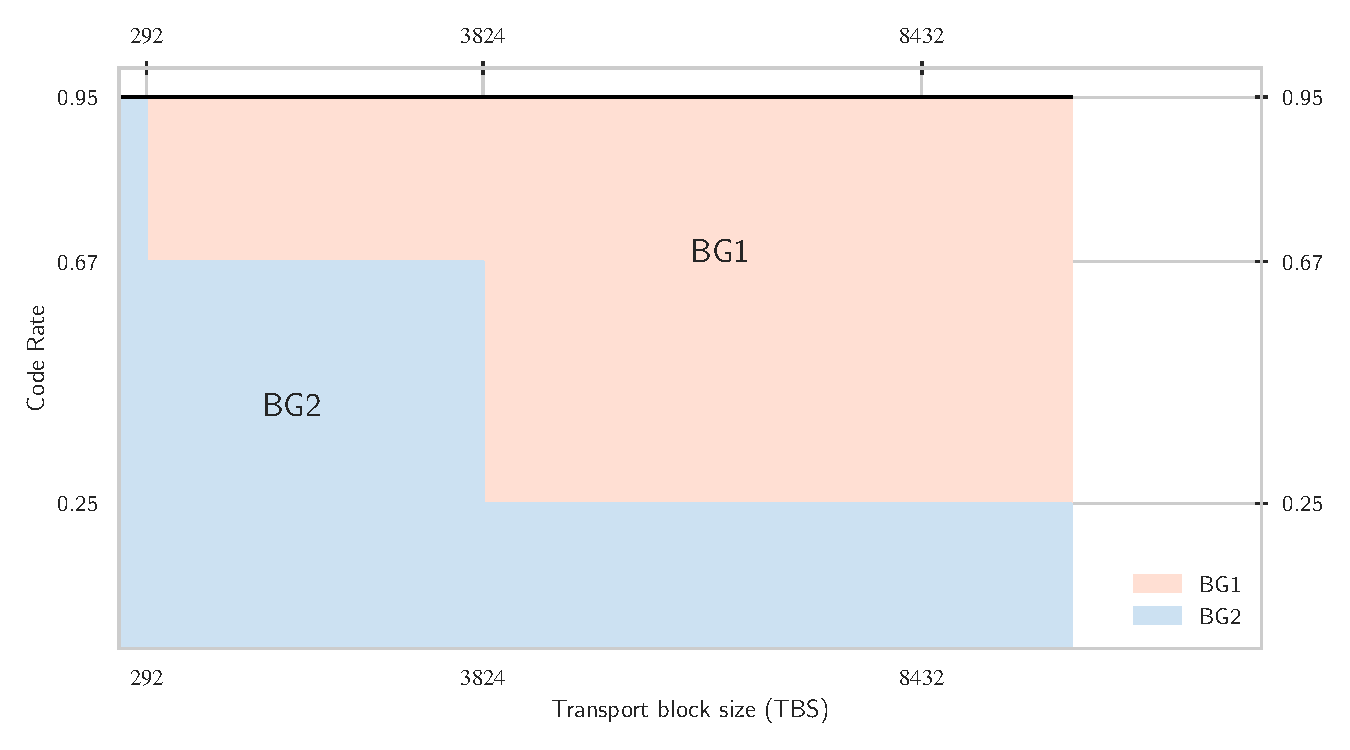
\includegraphics[width=\columnwidth]{figures/chp_theory/figureBG.pdf}
\caption{Base Graphs}
\source{Created by the author based on \cite{Hui2018}}
\label{fig:rate-vs-k}
\end{figure}

%%%%%%%%%%%%%%%%%%%%%%%%%%%%%--subsection--%%%%%%%%%%%%%%%%%%%%%%%%%%%%%%%%%
\subsection{\gls{crc} attachment and \gls{cb} segmentation}

The \gls{crc} bits are calculated from a cyclic generator polynomial.
%
In the \gls{pdsch} procedure there are three polynomials that can be used \cite{3gpp.38.212}:

\begin{equation} \label{eq.:crc24a}
    \begin{split}
        g_{\mathrm{CRC24A}}(D) = & [ D^{24} + D^{23} + D^{18} + D^{17} +  D^{14} + D^{10} \\ & + D^{7} + D^{7} + D^{5} + D^{4} + D^{3} + D + 1 ] \text{,}
    \end{split}
\end{equation}

\begin{equation}\label{eq.:crc24b}
    g_{\mathrm{CRC24B}}(D) = \left[ D^{24} + D^{23} + D^{6} + D^{5} + D + 1 \right] \text{and}
\end{equation}

\begin{equation} \label{eq.:crc16}
    g_{\mathrm{CRC16}}(D) = \left[ D^{16} + D^{12} + D^{5} + 1 \right] \text{.}
\end{equation}


The \gls{crc} makes possible for the receiver to detect errors in the decoded \gls{tb}.
%
For each \gls{tb} delivered from the \gls{mac} to the \gls{phy} a \gls{crc} is calculated and attached to it.
%
In case the \gls{tbs} is greater than 3824, the \gls{crc} has a length of 24 bits with the generator polynomial $g_{\mathrm{CRC24A}}$, Equation \eqref{eq.:crc24a}, being used.
%
Generator polynomial $g_{\mathrm{CRC16}}$, Equation \eqref{eq.:crc16}, is used otherwise, producing a 16-bit \gls{crc}.


\Gls{cb} segmentation occurs whenever the output of the \gls{crc} attachment is larger than the maximum code block size (8448 for \gls{bg} 1 and 3840 for \gls{bg} 2).
%
The objective of the segmentation is to produce \glspl{cb}, of equal size, that can be feed to the \gls{ldpc} encoder.
%
In the technical specification \cite{3gpp.38.212}, the \gls{cb} segmentation procedure is when the \gls{not:lift-factor} is selected.
%
The \glspl{cb} produced by the segmentation have size of $22 \gls{not:lift-factor}$ in case \gls{bg} 1 is used and $10 \gls{not:lift-factor}$ in case \gls{bg} 2 is used.
%
Filler bits are added whenever needed.

When \gls{cb} segmentation occurs each \gls{cb} receives a \gls{crc} of 24 bits, which is calculated from the generator polynomial $g_{\mathrm{CRC24B}}$, Equation \eqref{eq.:crc24b}.
%
This process is ilustrated in Figure \ref{fig:cbcrc}.
%
If only one \gls{cb} is produced, no additional \gls{crc} is attached to it \cite{ErikDahlman5G, 3gpp.38.212}.
%


\begin{figure}[htb]
    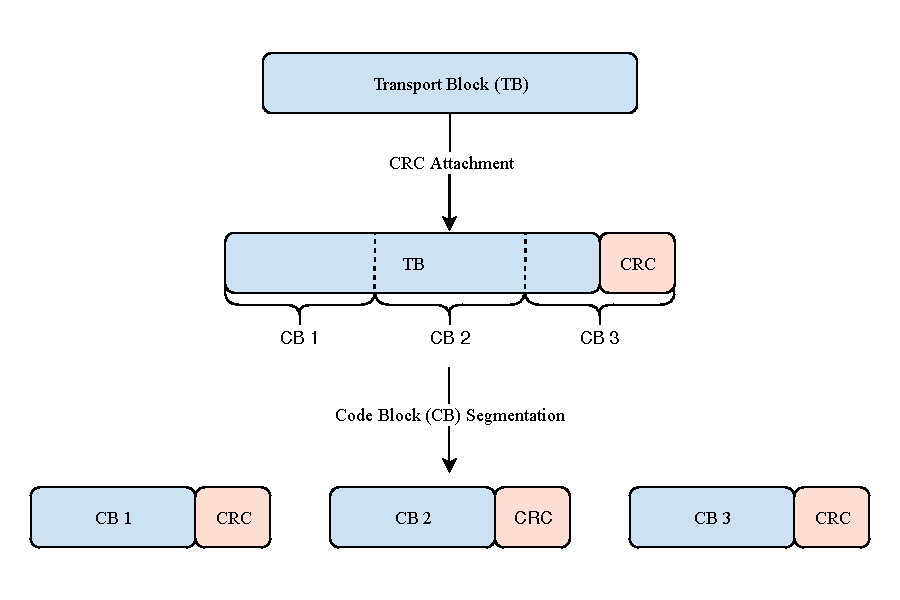
\includegraphics[width=\columnwidth]{figures/chp_theory/CRC.pdf}
    \caption{\gls{crc} attachements and \gls{cb} segmentation}
    \label{fig:cbcrc}
\end{figure}

%%%%%%%%%%%%%%%%%%%%%%%%--End Of subsection--%%%%%%%%%%%%%%%%%%%%%%%%%%%%%%

\subsection{\gls{ldpc} encoding}

The \glspl{cb} delivered after the \gls{cb} segmentation are then encoded as explained in \ref{subsec:ldpc}.
%
The size of the output of the encoder depends on the \gls{bg} selected \cite{3gpp.38.212}:
%
\begin{itemize}
    \item \gls{bg} 1: $66 \gls{not:lift-factor}$
    \item \gls{bg} 2: $50 \gls{not:lift-factor}$
\end{itemize}
%
Which means that the rate of the encoding process is the minimum designed code rate for each \gls{bg}:
%
\begin{itemize}
    \item \gls{bg} 1: rate of $\frac{1}{3}$
    \item \gls{bg} 2: rate of $\frac{1}{5}$
\end{itemize}

As explained in Section \ref{subsec:ldpc}, each non-zero element of the \gls{bg} is replaced by a circularly shifted identity matrix.
%
For the $(i,j)$th element of the \gls{bg}, the identity matrix is shifted to the right \gls{not:shift-coef} times.
%
The value of \gls{not:shift-coef} is given by:
%
\begin{equation}
    \gls{not:shift-coef} = \bmod (\gls{not:shift-value}, \gls{not:lift-factor}) ,
\end{equation}
%
\noindent where \gls{not:shift-value} is the $(i,j)$th element of the shift matrix specified in \cite[Tables 5.3.2-2 and 5.3.2-3]{3gpp.38.212} and it depends of the set index \gls{not:set-index}, which is dependent of the selected \gls{not:lift-factor}, as explained in Table \ref{tab:lift-table}.


%%%%%%%%%%%%%%%%%%%%%%%%--End Of subsection--%%%%%%%%%%%%%%%%%%%%%%%%%%%%%%

\subsection{Rate matching}

The rate matching is directly linked to the \gls{phy} \gls{harq} functionality, and they serve two purposes \cite{ErikDahlman5G}:
%
\begin{itemize}
    \item Select a suitable number of bits for transmission, matching the resources assigned for transmission.
    \item Support \gls{harq} by using different \glspl{rv}.
\end{itemize}
%
The rate matching consists of a bit selection from a circular buffer depending on of the \gls{rv} and each \gls{cb} is rate matched separately.

The \gls{5g} \gls{nr} \gls{ldpc} codes supports a circular buffer rate matching for \gls{irharq} similar to \gls{lte}.
%
The coded bits, which correspond to the output of the encoding step, are written in a circular buffer, the ordering of which follows the \gls{ldpc} matrix structure, with systematic bits first and then parity bits \cite{Hamidi8417496}.
%
The starting position of the bit selection in the circular buffer depends on the \gls{rv}, as shown in Figure \ref{fig:rate-match-rv}.
%
The \glspl{rv} fixed locations are defined in terms of the lifting value \gls{not:lift-factor} and are different for each \gls{bg}, as shown in Table \ref{tab:rv-positions} \cite{3gpp.38.212}.
%

\begin{table}[htb]
\centering
\caption{Starting positions for each \gls{rv} and \gls{bg}}
\label{tab:rv-positions}
\begin{tabularx}{0.55\columnwidth}{l c c c r}
  \toprule
  \Gls{bg}  & \gls{rv} 0  & \gls{rv} 1 & \gls{rv} 2 & \gls{rv} 3   \\
  \midrule
  \Glsentrylong{bg} 1 & $0$ & $17 \gls{not:lift-factor}$ & $33 \gls{not:lift-factor}$ & $56 \gls{not:lift-factor}$\\
  \Glsentrylong{bg} 2 & $0$ & $13 \gls{not:lift-factor}$  & $25 \gls{not:lift-factor}$ & $43 \gls{not:lift-factor}$\\
  \bottomrule
\end{tabularx}
\end{table}


Selecting different \glspl{rv} enables the receiver to apply soft-combining by keeping the soft values of the received coded bits, i.e the \glspl{llr}, and combining it with the retransmitted bits, in case of a retransmission.
%
Since each retransmission corresponds to a different \gls{rv}, multiple \glspl{cb} are generated, representing the same set of information, which enables different parity bits to be transmitted at each retransmission, as illustrated in figure Figure \ref{fig:rate-match-rv}.
%
This allows a gain in reliability, not only because of the better estimation of the soft values, but also thanks to the lower rate of the resultant soft combined values \cite{ErikDahlman5G,bae_abotabl_lin_song_lee_2019}.


\begin{figure}[htb]
    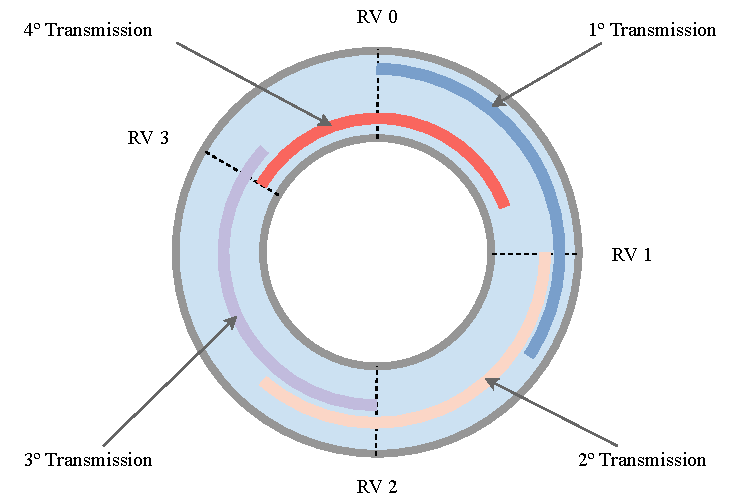
\includegraphics[width=0.8\columnwidth]{figures/chp_theory/rate-matching-rv.pdf}
    \caption{Example of different \gls{rv} positions and retransmissions}
    \label{fig:rate-match-rv}
    \source{Created by the author based on \cite[Figure 9.5]{ErikDahlman5G}}
\end{figure}


Although the procedure applied in this work only concerns the \gls{ldpc} rate matching, we highlight the more general procedure of the polar coding rate matching.
%
In \cite{Hui2018} three different cases are defined: puncturing, shortening and repetition.
%
We denote the input to the polar coding rate matching as \gls{not:coded-bits} and the desired length of the output as \gls{not:rm-bits}.
%
Puncturing and shortening refer to the case of $\gls{not:coded-bits} > \gls{not:rm-bits}$, while repetition refers to the case of $\gls{not:coded-bits} < \gls{not:rm-bits}$, then:
%
\begin{enumerate}
    \item Puncturing: Extracting \gls{not:rm-bits} bits starting from the $(\gls{not:coded-bits} - \gls{not:rm-bits} + 1)$th bit on the circular buffer. This is equivalent to selecting the last \gls{not:rm-bits} bits of the circular buffer.
    %
    \item Shortening: Extracting \gls{not:rm-bits} bits starting from the initial position on the circular buffer. This is equivalent to selecting the first \gls{not:rm-bits} bits of the circular buffer.
    %
    \item Repetition: Extracting \gls{not:rm-bits} bits starting from the initial position on the circular buffer while wrapping around on the last $(\gls{not:coded-bits} - \gls{not:rm-bits})$ bits. This is equivalent to selecting all the \gls{not:coded-bits} bits of the circular buffer and adding the first $(\gls{not:coded-bits} - \gls{not:rm-bits})$ again.
\end{enumerate}
%
All these cases are illustrated in Figure \ref{fig:rate-matching}:

\begin{figure}[htb]
    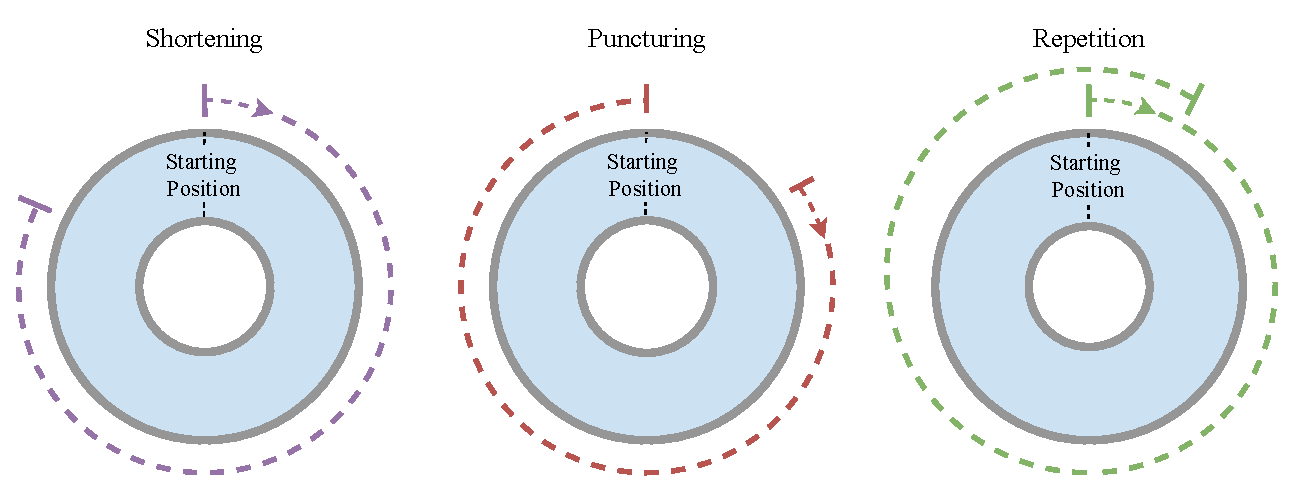
\includegraphics[width=\columnwidth]{figures/chp_theory/rate-matching.pdf}
    \caption{Rating matching methods for polar coding}
    \label{fig:rate-matching}
\end{figure}

\Gls{ldpc} rate matching includes only the shortening and repetition equivalents of the polar coding rate matching, although the shortening of the polar codes is equivalent to the so called puncturing of the \gls{ldpc} in \cite{Hui2018}.
%
Hence, is possible to call simply bit selection, as in \cite{3gpp.38.212}, since both the puncturing and repetition procedures select the bits starting from the initial position given by the \gls{rv}, the difference is that repetition is defined for $\gls{not:coded-bits} < \gls{not:rm-bits}$ and the \gls{ldpc} equivalent of shortening is defined for $\gls{not:coded-bits} > \gls{not:rm-bits}$.

The rate matching also includes the interleaving step, and it is applied to each \gls{cb} separately.
%
A row-column block interleaver is used in \gls{nr} \gls{ldpc}, the number of rows being equal to the modulation order.
%
The writing of the bits in the interleaver is made row-by-row, while the reading of the bits is made column-by-column.
%
It is important to notice that the bits in one column correspond to one modulation symbol \cite{Hamidi8417496,ErikDahlman5G}.

%%%%%%%%%%%%%%%%%%%%%%%%--End Of subsection--%%%%%%%%%%%%%%%%%%%%%%%%%%%%%%
\subsection{Layer mapping}

The modulated symbols are distributed across the different transmission layers.
%
One \gls{tb} can be mapped to a maximum of 4 layers, as stated in  \cite[Table 7.3.1.3]{3gpp.38.211}.
%
In case of 5 to 8 layers (only on downlink) another \gls{tb} is mapped to layers from 5 to 8.
%
The mapping respects a one-to-one correspondence, i.e., every n-th symbol is mapped to the n-th layer \cite{ErikDahlman5G}.

As an example, we show the cases of 3, 5 and 6 layers.
%
For a sequence of symbols $d^{(q)}$ modulated from the $q$-th \gls{tb} and with
$\gls{not:nLayers}_q$ being the number of layers allocated to the transmission of the $q$-th \gls{tb} and $x$ being the output of the layer mapping, where $x^{(j)}$ is the vector of complex symbols mapped to layer $j$, we have:
%
\begin{itemize}
    \item $\gls{not:nLayers} = 3 $, then $q=0$ and $\gls{not:nLayers}_q = 3$:
    $$
    \begin{gathered}
        x^{(0)}_{i} = d^{(0)}_{3 i} \\
        x^{(1)}_{i} = d^{(0)}_{3 i + 1} \\
        x^{(2)}_{i} = d^{(0)}_{3 i + 2}
    \end{gathered}
    $$
    \item $\gls{not:nLayers} = 5 $, then $q \in \{0,1\}$, $\gls{not:nLayers}_0 = 2$ and $\gls{not:nLayers}_1 = 3$:
    $$
    \begin{gathered}
        x^{(0)}_{i} = d^{(0)}_{2 i} \\
        x^{(1)}_{i} = d^{(0)}_{2 i + 1} \\
        x^{(2)}_{i} = d^{(1)}_{3 i} \\
        x^{(3)}_{i} = d^{(1)}_{3 i + 1} \\
        x^{(4)}_{i} = d^{(1)}_{3 i + 2}
    \end{gathered}
    $$
    \item $\gls{not:nLayers} = 6 $, then $q \in \{0,1\}$, $\gls{not:nLayers}_0 = 3$ and $\gls{not:nLayers}_1 = 3$:
    $$
    \begin{gathered}
        x^{(0)}_{i} = d^{(0)}_{3 i} \\
        x^{(1)}_{i} = d^{(0)}_{3 i + 1} \\
        x^{(2)}_{i} = d^{(0)}_{3 i + 2} \\
        x^{(3)}_{i} = d^{(1)}_{3 i} \\
        x^{(4)}_{i} = d^{(1)}_{3 i + 1} \\
        x^{(5)}_{i} = d^{(1)}_{3 i + 2}
    \end{gathered}
    $$
\end{itemize}

We can generalize this mapping via the following expression:
%
\begin{equation}
    x^{(j)}_{i} =
    \begin{cases}
          d^{(0)}_{\gls{not:nLayers}_0 i + j} \text{ , for } j=0,\ldots, \gls{not:nLayers}_0 - 1 \\
         d^{(1)}_{\gls{not:nLayers}_1 i + j} \text{ , for } j=\gls{not:nLayers}_0, \ldots, \gls{not:nLayers} - 1
    \end{cases}
\end{equation}


%
With more than 4 layers the number of layers assigned to the transmission of each \gls{tb} is:
\begin{equation}
    \begin{gathered}
        \gls{not:nLayers}_0 = \floor{\gls{not:nLayers}/2} \\
        \gls{not:nLayers}_1 = \ceil{\gls{not:nLayers}/2}
    \end{gathered}
\end{equation}


%%%%%%%%%%%%%%%%%%%%%%%%--End Of subsection--%%%%%%%%%%%%%%%%%%%%%%%%%%%%%%
\subsection{Multi-antenna Precoding}

In the multi-antenna precoding step, the different transmission layers are mapped to a set of antenna ports by a precoder matrix.
%
The definition of antenna port given in the technical specification \cite{3gpp.38.211} is ``an antenna port is defined such that the channel over which a symbol on the antenna port is conveyed can be inferred from the channel over which another symbol on the same antenna port is conveyed''\cite[Section 4.4.1]{3gpp.38.211}.
%
This means that, every downlink transmission is executed by a specific antenna port, with its identity known to the \gls{ue} and that the \gls{ue} can assume that two transmitted signals shared the same radio channel if and only if they used the same antenna port \cite{ErikDahlman5G, AliZaidi632018}.
%

It is important to note that antenna port is an abstract concept, as it is a logical entity that does not correspond necessarily to a specific physical antenna.
%
In practice what defines an antenna port is the transmitted reference signal, since the \gls{ue} can use a reference signal, such as the \gls{dmrs}, conveyed by an antenna port to estimate the channel of this antenna port and use this estimate to decode the data transmitted by the same antenna port afterwards.
%
To illustrate what this means, we highlight two examples based on \cite{ErikDahlman5G, AliZaidi632018}:
\begin{itemize}
    \item In the case that multiple physical antennas transmit two different signals in the same way, the \gls{ue} will perceive these two signals as being propagated by the same single channel, which corresponds to the combination of the channels of the different physical antennas. The \gls{ue} will see these two signals as if they were transmitted from the same antenna port.

    \item In the case that two signals are transmitted from the same set of physical antennas and beam-formed with different weights, the resulting transmission will be considered as being from two different antenna ports, because the \gls{ue} will perceive two different effective channels, since the precoder is unknown to the \gls{ue}.
\end{itemize}

Table \ref{tab:antenna-ports} shows the defined sets of antenna ports for \gls{5g} \gls{nr} and their respective usages in the downlink and uplink \cite[Subsections 6.2 and 7.2]{3gpp.38.211}, which include a number of reference signals, such as the \gls{csi}-\gls{rs}, \gls{ss} and \gls{srs}.

\begin{table}[htb]
\centering
\caption{Antenna ports}
\label{tab:antenna-ports}
\begin{tabular}{l c c}
  \toprule
  Antenna port series & Uplink & Downlink \\
  \midrule
  Starting with 0  &  \gls{dmrs} for \gls{pusch} & \textemdash \\
  Starting with 1000  & \gls{srs}, \gls{pusch} & \gls{pdsch}   \\
  Starting with 2000  & \gls{pucch} & \gls{pdcch} \\
  Starting with 3000  & \textemdash & \gls{csi}-\gls{rs} \\
  Starting with 4000  & \gls{prach} & \gls{ss}/\gls{pbch} block transmission \\
  \bottomrule
\end{tabular}
\end{table}

The mapping between the \gls{not:nLayers} layers and the $\gls{not:txAnt}_{\text{AP}}$ antenna ports is defined by a $\gls{not:txAnt}_{\text{AP}} \times \gls{not:nLayers}$ precoder matrix \gls{not:Wtx}.
%
This mapping is specification-transparent, since the \gls{ue} can assume that the \glspl{dmrs} are precoded hand in hand with the data as shown in Figure \ref{fig:precoder-dmrs}.
%
Therefore, the choice of the precoder is up to the network implementation and is transparent to the \gls{ue} \cite{8928165, ErikDahlman5G}.

\begin{figure}[htb]
    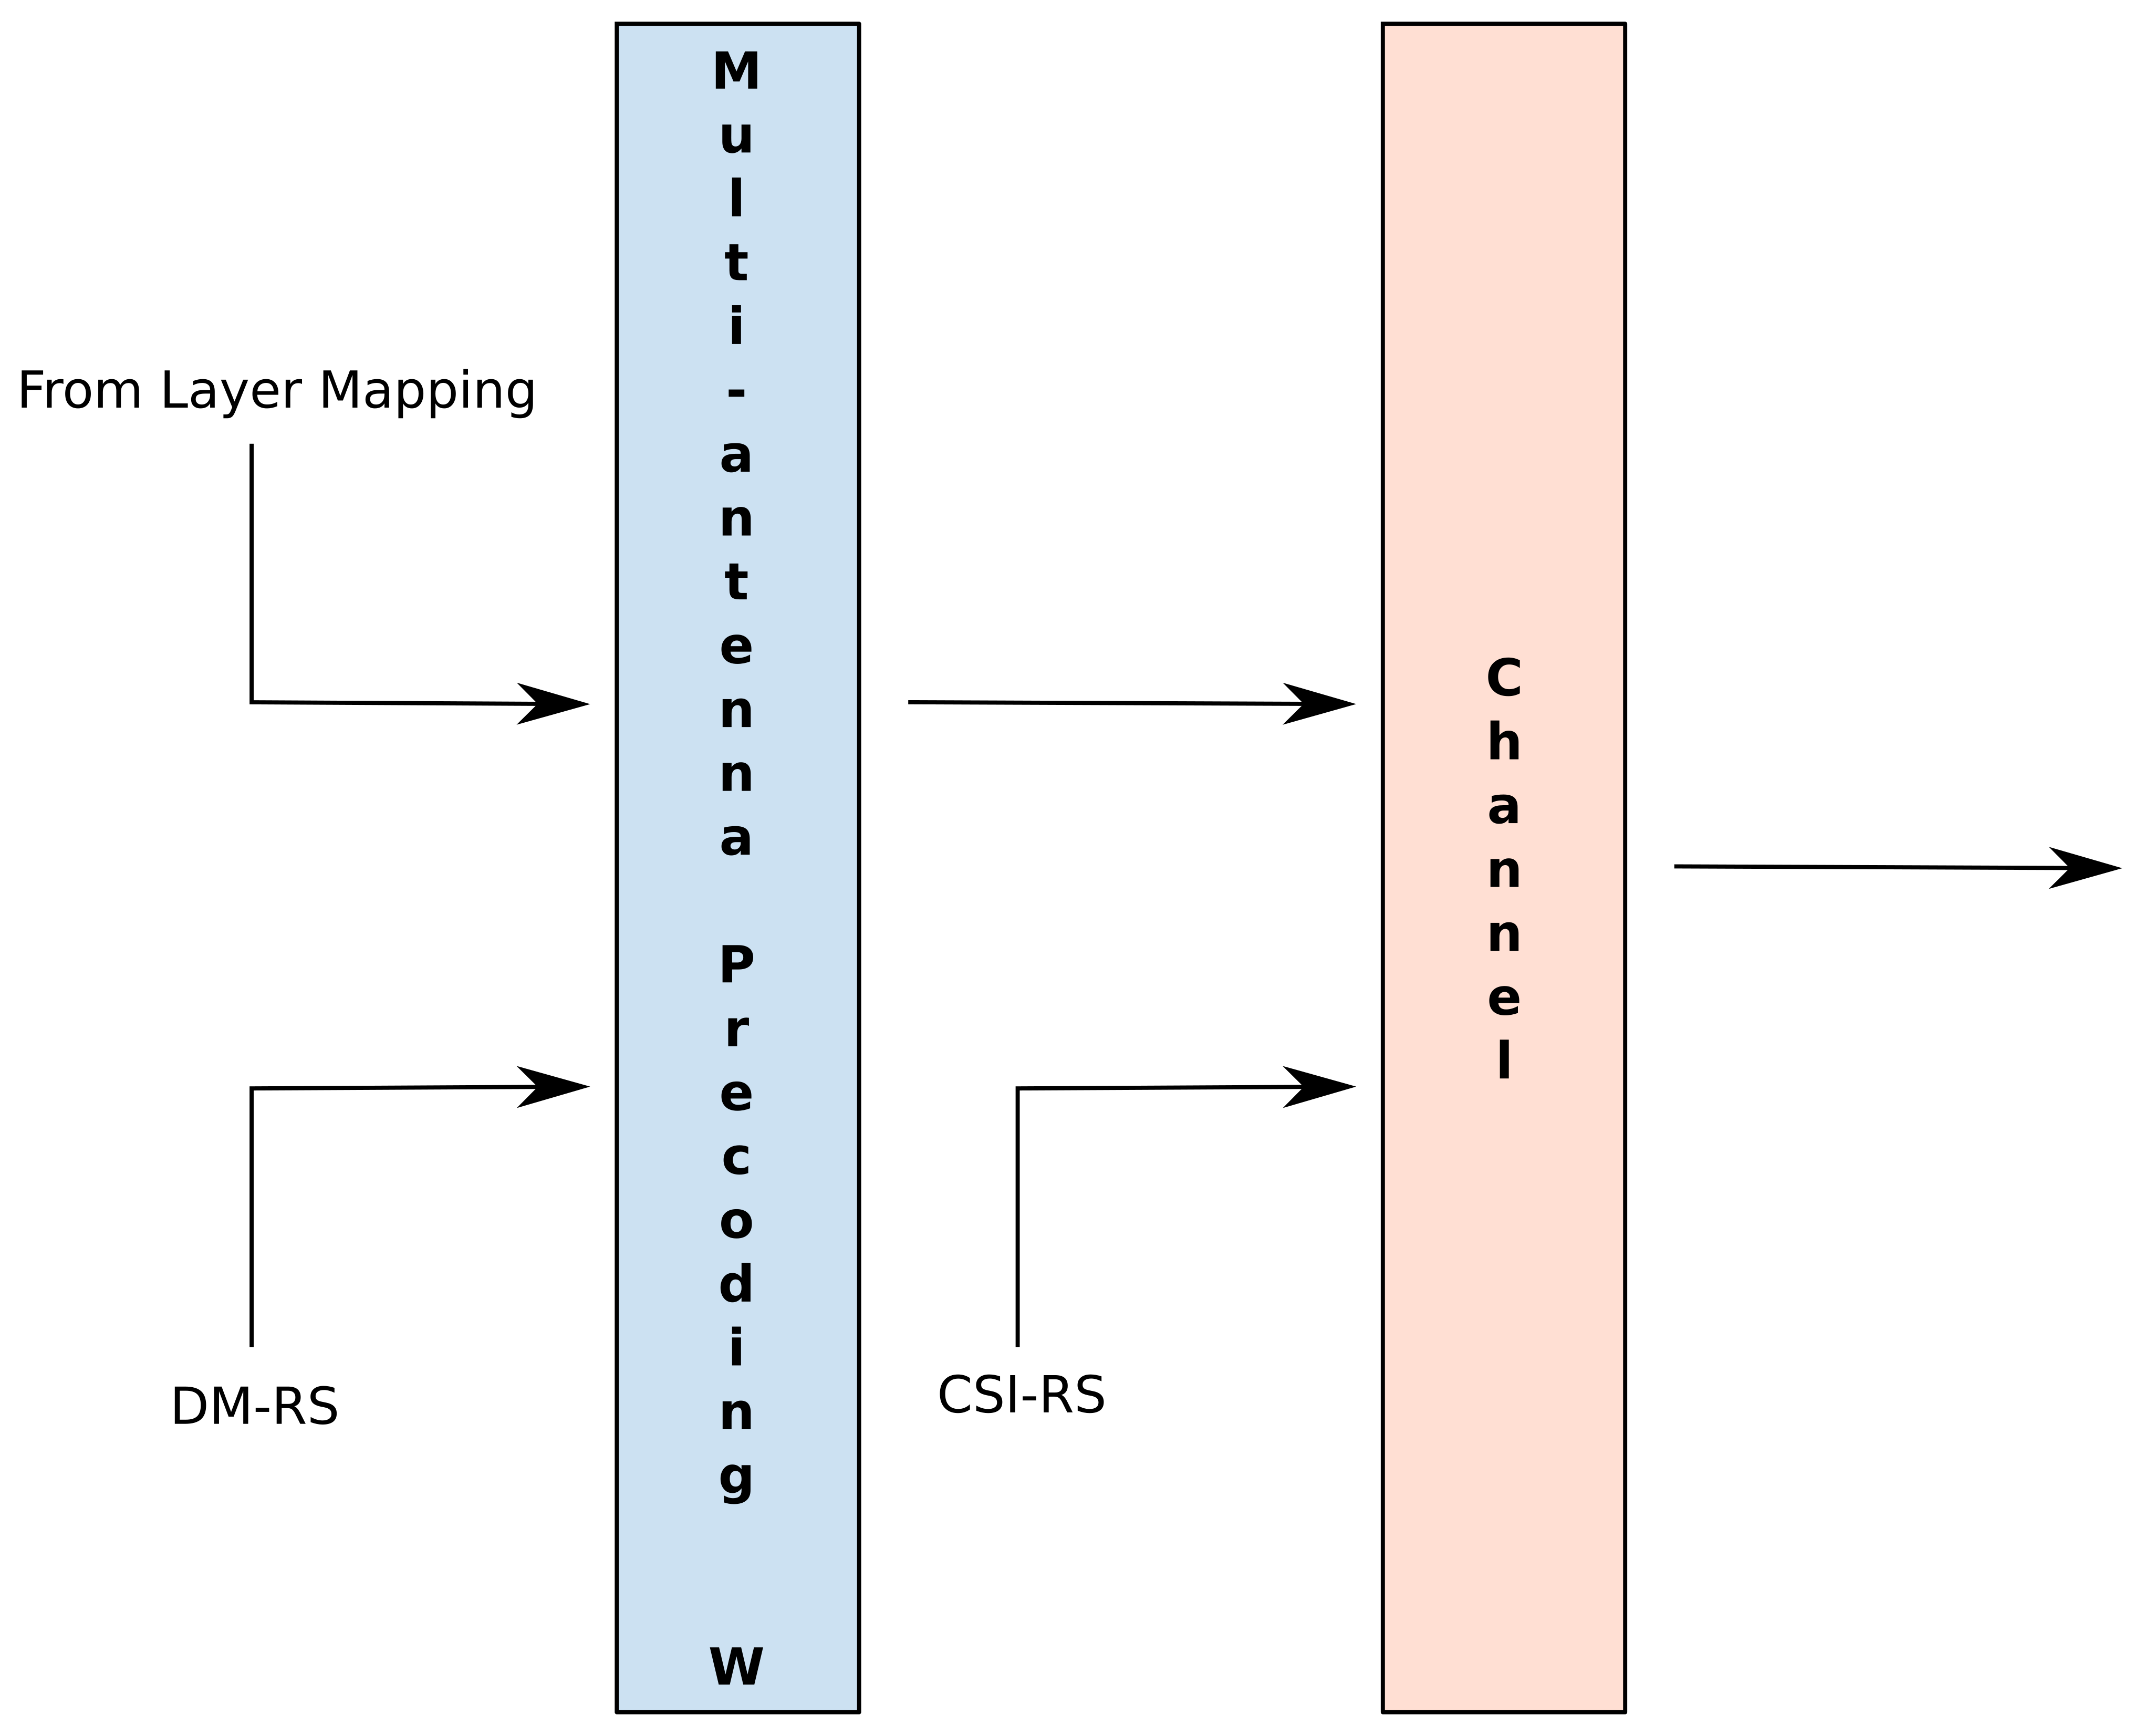
\includegraphics[width=0.5\columnwidth]{figures/chp_theory/figchannel.png}
    \caption{Downlink precoding and reference signals. }
    \label{fig:precoder-dmrs}
\end{figure}

The selection of the precoder by the network is supported by the reporting of some information by the \gls{ue}, which are part of the \gls{csi} report.
%
The most important reference signal to compute the \gls{csi} is the \gls{csi}-\gls{rs}, which is shown in Figure \ref{fig:precoder-dmrs}.
%
The quantities in the \gls{csi} report more relevant to this work are \cite{AliZaidi632018}:
%
\begin{enumerate}
    \item \Gls{ri}: The preferred transmission rank, number of layers, to use in a codebook-based precoded downlink transmission.
    \item \Gls{pmi}: Indicates the preferred precoder matrix, given the selected rank.
    \item \Gls{cqi}: Index to the preferred \gls{mcs}, which is the highest \gls{mcs} that gives a \gls{bler} of 0.1 in case \gls{cqi} Tables 1 and 2 \cite[Tables 5.2.2.1-2 \& 5.2.2.1-3]{3gpp.38.214} or a \gls{bler} of 0.00001 in the case of \gls{cqi} Table 3 \cite[5.2.2.1-4]{3gpp.38.214}, given the selected precoder and rank.
\end{enumerate}

The \gls{pmi} indicates the precoder matrix that the \gls{ue} believes to be the best option from a set of precoders of the codebook.
%
Since the device selects the precoder based on a certain number of antenna ports and a number of layers (selected transmission rank), each combination of $\gls{not:txAnt}_{\text{AP}}$ and $\gls{not:nLayers}$ represents at least one codebook.
%
The \gls{pmi} only indicates the precoder that the \gls{ue} prefers, i.e it imposes no restriction on the precoder selection from the network for downlink transmissions \cite{ErikDahlman5G, AliZaidi632018}.
%
Nevertheless, at Chapter \ref{chp:la} only the codebooks and precoders defined in \cite{3gpp.38.214} are used.
%
The precoders for 2 antenna-ports and for one and two layer transmission are shown in Figure \ref{fig:precoder-codebook}.

\begin{figure}[htb]
    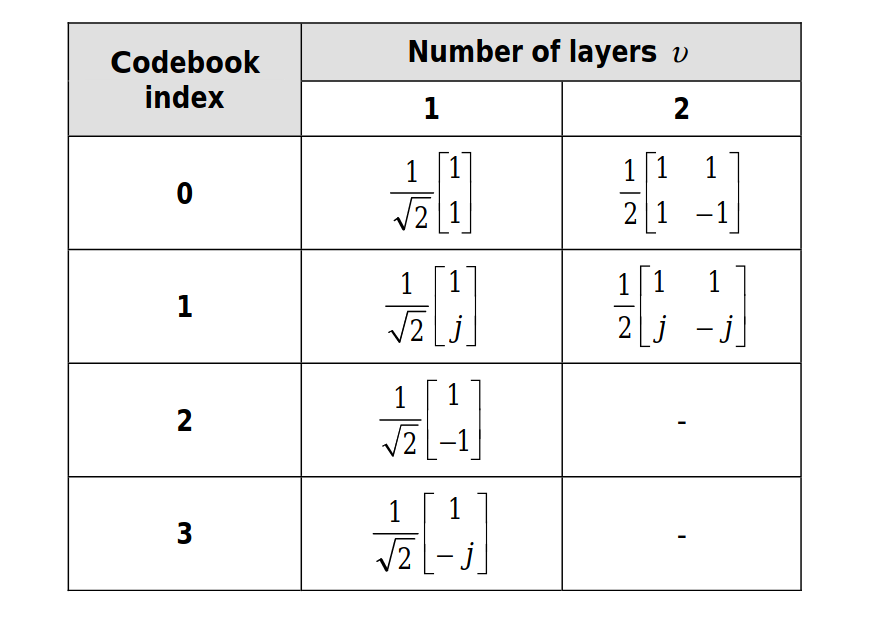
\includegraphics[width=0.7\columnwidth]{figures/chp_theory/Precoders_codebook.png}
    \caption{Type I Single Panel Codebooks for 2 antenna ports. }
    \label{fig:precoder-codebook}
    \source{\cite[Table 5.2.2.2.1-1]{3gpp.38.214}}
\end{figure}


%%%%%%%%%%%%%%%%%%%%%%%%--End Of subsection--%%%%%%%%%%%%%%%%%%%%%%%%%%%%%%

\subsection{Downlink Transmission and Link Adaptation}

% In this subsection the subsections above are summarized and contextualized with the \gls{la} problem.
The downlink \gls{mimo} transmission uses two main reference signals, the \gls{csi}-\gls{rs} and the \gls{dmrs}.
%
\Gls{csi}-\gls{rs} is mainly used for \gls{csi} acquisition and it can be beamformed or transmitted per antenna element.
%
Then, the \gls{ue} can estimate the channel and send its \gls{csi} report, consisting of information, such as \gls{ri}, \gls{pmi} and \gls{cqi}.
%
In possession of the feedback from the \gls{ue}, the \gls{bs} can select the best parameters for downlink transmission, and inform some important information to the \gls{ue}, such as the \gls{mcs} and \gls{ri}, and performs the data transmission \cite{AliZaidi632018}.

The link adaptation is the choice of some of these transmission parameters, in our case mainly the \gls{mcs} in Chapter \ref{chp:amc} and the \gls{mcs} and precoder (therefore the \gls{ri}) in Chapter \ref{chp:la} by means of reinforcement learning.

%%%%%%%%%%%%%%%%%%%%%%%%--End Of Section--%%%%%%%%%%%%%%%%%%%%%%%%%%%%%%
\section{Reinforcement Learning }
\label{sec:rl-theory}
\Gls{rl} is a \gls{ml} technique that aims to find the best behavior in a given situation in order to maximize a notion of accumulated reward \cite{Bishop07,survey-son}.
%
Figure \ref{fig:rlbasic} shows a simple block diagram of the \gls{rl} problem in which an agent, which is the learner and decision maker, interacts with an environment by taking actions.
%
By its turn, the environment responds to these actions and presents new situations, as states, to the agent \cite{sutton2018rl}.
%
The environment also responds by returning rewards, which the agent tries to maximize by choosing its actions.
%
Unlike supervised learning, where the system learns from examples of optimal outputs, the \gls{rl} agent learns from trial and error, i.e., from its experience, by interacting with the environment.

\begin{figure}[htbp]
\centerline{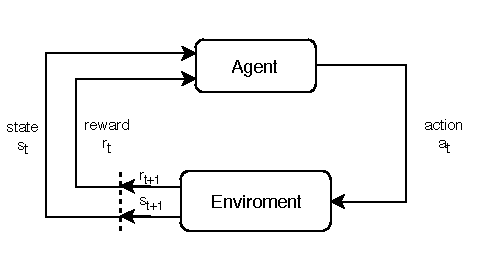
\includegraphics[width=90mm]{figures/chp_theory/rl-model.pdf}}
\caption{Basic diagram of a \gls{rl} scheme}
\label{fig:rlbasic}
\end{figure}
% another intro:
% Reinforcement Learning (RL) is a machine Learning tech-
% nique that aims to find the best behavior in a given situation
% in order to maximize a notion of accumulated reward [8].
% Figure 1 shows a simple block diagram of RL problem, in
% which an agent interacts with an environment by taking actions
% and evaluating the results of these actions, these results are
% perceived by the agent as a new state and by a received reward
% signal. Unlike supervised learning, where the system learns
% from examples of optimal outputs, the RL agent learns from
% trial and error.

At each time step $t$, the agent receives the state of environment $s_t \in \mathcal{S}$, and based on that chooses an action $a_t \in \mathcal{A}$.
%
As consequence of its action, the agent receives a reward $r_{t+1} \in \mathcal{R} $, with $\mathcal{R} \subset \mathbb{R}$, and perceives a new state $s_{t+1}$.
%
In light of this, the basics components of a \gls{rl} problem are:

\begin{itemize}
  \item State Space $\mathcal{S}$: Set of all possible states that can be observed by the agent. The random variable $S_t$ denotes the state at time step $t$ and a sample of $S_t$ is denoted $s_t$, with $s_t \in \mathcal{S}$.
  \item Action Space $\mathcal{A}$: Set of all actions that can be taken by the agent. The random variable $A_t$ denotes the action at time step $t$ and a sample of $A_t$ is denoted $a_t$, with $a_t \in \mathcal{A}$
  \item Transition Probability Space $\mathcal{P}: \mathcal{S} \times \mathcal{A} \times \mathcal{S} \rightarrow [0;1]$ is the transition model of the system, $p(s_{t+1} | s_t,a_t) \in \mathcal{P}$ is the probability of transitioning to state $s_{t+1}$ after taking action $a_t$ in state $s_t$.
  \item Reward  $r_t$: This value indicates the immediate payoff from taking an action $a_{t-1}$ in a state $s_{t-1}$. $R_t$ is a random variable with a probability distribution depending only of the preceding state and action. We define the expected reward obtained from taking an action $a_t$ in a state $s_t$ as $r(s_t,a_t) = \mathbb{E}\left[R_{t+1} \, | \, S_t = s_t, A_t = a_t \right] $.
  \item Policy $\pi(s_t) \in \mathcal{A} $: The policy maps the states to actions. More specifically, it maps the perceived states of the environment to the actions to be taken by the agent in those states. The policy can also be defined as $\pi(a_t | s_t)$, the probability of selecting action $a_t$ given the agent is at a state $s_t$.
  % different policies can give different probabilities to each action.
  \item Q-function $Q^{\pi}(s_t,a_t)$:  The Q-Function, called action-value function, is the overall expected reward for taking an action $a_t$ in a state $s_t$ and then following a policy $\pi$. It can also be simply denoted as $Q(s_t,a_t)$.
\end{itemize}


The goal of the \gls{rl} agent is to find the optimal policy $\pi^{*}(s_t)$, whose state-action mapping leads to the maximum long term discounted reward given by $G_t = \sum_{k=0}^{\infty} \gamma^{k} R_{t+k+1} = R_{t+1} + \gamma G_{t+1} $ \cite{kaelbling1996reinforcement}.
% , where $r_t$ is the received reward at time step $t$.
%
The agent finds its best policy by taking into consideration the value of the Q-function to a state-action pair.
%
Mathematically, the Q-Function is defined as \cite{2010Szepesvari}:
\begin{equation} \label{eq.:eqQvalue}
  Q^{\pi}(s_t, a_t) \doteq \mathbb{E}\left[\sum_{k=0}^{\infty} \gamma^{k} R_{t+k+1} \, | \, S_t = s_t, A_t = a_t \right], s_t \in \mathcal{S}, a_t = \pi (s_t) \in \mathcal{A}.
\end{equation}


The parameter $\gamma$ is called \textit{discount factor}, or discount rate, with $0 \leq \gamma < 1$.
%
The discount factor is used to control the importance given to future rewards in comparison with immediate rewards, so a reward received $k$ time steps later is worth only $\gamma^{k-1}$ times its value.
%
The infinity sum $\sum_{t=0}^{\infty} \gamma^{t} r_{t+1}$ has a finite value if $\gamma \leq 1$, as long as the sequence $\{r_k\}$ is bounded \cite{sutton2018rl}.
%
The process is called undiscounted if $\gamma=1$.


The Q-values in successive steps are related according to the Bellman equation:
\begin{equation} \label{eq.:bellmanEq}
  %\begin{split}
    Q^{\pi}(s_t, a_t)= \sum_{s_{t+1} \in \mathcal{S}} p\left(s_{t+1} \, | \, s_t , a_t \right) \bigg[ r\left(s_t, a_t \right)  +
    \gamma \sum_{a_{t+1} \in \mathcal{A}} \pi\left(a_{t+1} \, | \, s_{t+1}\right) Q^{\pi}\left(s_{t+1}, a_{t+1}\right)  \bigg] \text{.}
  %\end{split}
\end{equation}

The Equations \eqref{eq.:eqQvalue} and \eqref{eq.:bellmanEq} can be rewritten for the case of $\pi$ being the optimal policy.
%
In this case, Equation \eqref{eq.:eqQvalue} leads to \cite{sutton2018rl}:

\begin{equation} \label{E_Optimal}
    Q^{\pi^*}\left(s_t, a_t\right)=\mathbb{E}\left[R_{t+1}+\gamma \max _{a^\prime \in \mathcal{A}} Q^{\pi^*}\left(S_{t+1}, a^\prime \right) \, | \, S_t=s_t, A_t=a_t\right] \text{.}
\end{equation}

Likewise, assuming the optimal policy, Equation \eqref{eq.:bellmanEq} leads to \cite{DRL_AMC}:

\begin{equation} \label{eq.:bellmanOptimal}
    Q^{\pi^*}\left(s_t, a_t\right)=r(s_t,a_t)+ \gamma \sum_{s_{t+1} \in \mathcal{S}} p\left(s_{t+1} \, | \, s_t,a_t\right) \max _{a^\prime \in A} Q^{\pi^*}\left(s_{t+1}, a^\prime \right) \text{.}
\end{equation}


Equation \eqref{eq.:bellmanOptimal} can only be solved if we know the transition probabilities.
%
However, if we don't have an adequate model of the environment the agent can take actions and observe their results, then it can fine-tune the policy that decides the best action for each state.
%
The algorithms that explore the environment to find the best policy are called model-free, while those ones that use the transition probabilities are called model-based.


\subsection{Exploration and Exploitation Trade-off}

One of the main paradigms in \gls{rl} is the balancing of exploration and exploitation.
%
The agent is exploiting if is choosing the action that has the greatest estimate of action-value, these are usually called the greedy actions.
%
Whereas exploring is when the agent chooses the non-greedy actions, to improve their estimates.
%
This leads to a better decision-making because of the information the agent has about these non-greedy actions \cite{sutton2018rl}.
%


There are different strategies to control the exploring and exploiting trade off. The reader have a deep discussion on that topic in \cite{exploration2016}.
%
In this work, we make use of the first two strategies:
\begin{enumerate}
  \item $\epsilon$-greedy: One of the most common exploration strategies. It selects the greedy action with probability $1-\epsilon$, and a random action with probability $\epsilon$. So, a higher $\epsilon$ means that the agent gives more importance to exploration.
  \item adaptive $\epsilon$-greedy: There are numerous different methods that adapt the $\epsilon$ over time or as a function of the error \cite{improvingBandits}. A commonly used approach is to start with a high $\epsilon$ and decrease it over time.
  \item Boltzmann exploration: Also known as softmax exploration. It uses the action-values to choose an action according to the Boltzmann distribution:
  \begin{equation}
      \pi\left(s, a\right)=\frac{e^{Q\left(s, a\right) / T}}{\sum_{i=1}^{m} e^{Q\left(s^{\prime}, a_i\right) / T}} \text{.}
  \end{equation}

  The parameter $T \geq 0$, called temperature, sets the balance between exploration and exploitation. If $T \rightarrow 0$  the agent will only exploit, if $T \rightarrow \infty$ the agent will choose actions at random.
\end{enumerate}


\subsection{Q-Learning}

In this work, we adopt the Q-learning algorithm, which is an off-policy temporal difference (TD) algorithm.
%
TD methods are model-free and they update their estimates partially based on other estimates, without the need to wait for a final outcome \cite{sutton2018rl}.
%
An off-policy method can learn about the optimal policy at the same time it follows a different policy, called the behavior policy.
%
This behavior policy still has an effect on the algorithm, because it determines the choices of actions. The basic form of the action-values updates is:
\begin{equation}\label{QlearningEq}
%  \begin{split}
    Q\left(s_{t}, a_{t}\right) \leftarrow  (1-\alpha) Q\left(s_{t}, a_{t}\right)
    +\alpha\left[r_{t+1}+\gamma \max _{a_{t+1} \in A} Q\left(s_{t+1}, a_{t+1}\right)\right],
%  \end{split}
\end{equation}

\noindent where the parameter $0 \leq \alpha \leq 1$ is called learning rate.

The Algorithm \ref{alg1} details Q-learning algorithm \cite{sutton2018rl}.

\begin{algorithm}[!t]

Algorithm parameters: step size $\alpha \in (0, 1]$, small $\epsilon > 0$\;
Initialize $Q(s, a)$, for all $s \in \mathcal{S}, a \in \mathcal{A}$\;
\ForEach{iteration}{
Initialize s\;
  Choose $a$ from $s$ using policy derived from $Q$ (e.g., $\epsilon$-greedy)\;
  Take action $a$, observe $r$, $s^{\prime}$\;
  $Q(s, a) \leftarrow (1-\alpha) Q(s, a) + \alpha [r + \gamma \max_{a^\prime} Q(s',a^\prime)]$\;
  $s \leftarrow s^{\prime}$\;

}
\caption{Q-learning (off-policy TD control) for estimating $\pi \approx \pi^* $}
  \label{alg1}
\end{algorithm}

In the next chapters, the basic Q-learning framework described in this section is applied to two different problems.
%
In Chapter \ref{chp:amc}, we investigate a Q-learning based \gls{amc} algorithm.
%
In Chapter \ref{chp:la}, we address the link adaptation problem for \gls{5g} \gls{nr} from the perspective of Q-learning.
